%% LyX 2.2.2 created this file.  For more info, see http://www.lyx.org/.
%% Do not edit unless you really know what you are doing.
\documentclass[spanish]{article}
\usepackage[T1]{fontenc}
\usepackage[latin9]{luainputenc}
\usepackage{array}
\usepackage{float}
\usepackage{textcomp}
\usepackage{multirow}
\usepackage{graphicx}

\makeatletter

%%%%%%%%%%%%%%%%%%%%%%%%%%%%%% LyX specific LaTeX commands.
%% Because html converters don't know tabularnewline
\providecommand{\tabularnewline}{\\}

\makeatother

\usepackage{babel}
\addto\shorthandsspanish{\spanishdeactivate{~<>}}

\begin{document}

\section{Ejercicio 3}

\subsection{Consigna}

En este ejercicio se implementar� una maquina de estados de Moore
siguiendo lo solicitado por el trabajo y luego se har� una maquina
de estados equivalente en su versi�n Mealy. Esta maquina de estados
es la que se muestra a continuaci�n:

\begin{figure}[H]
\begin{centering}
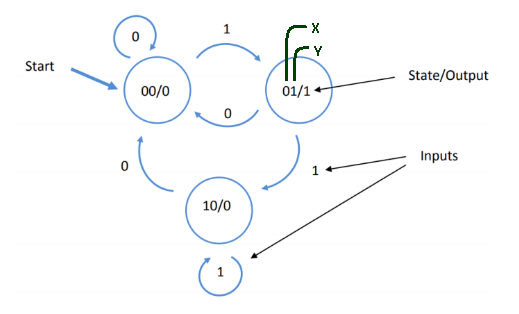
\includegraphics[width=10cm,height=10cm,keepaspectratio]{imagenes/consigna}
\par\end{centering}
\caption{Maquina de estados solicitada}

\end{figure}


\subsection{Maquina de estado de Moore}

Como se sabe las maquinas de estado de Moore se caracterizan por tener
una salida unicamente dependiente del estado actual del sistema, sin
depender de forma instant�nea de la entrada.

Como\ primera instancia para resoluci�n de esta maquina se define
que valores para los bits denominados como \emph{X} e \emph{Y }caracterizan
a cada uno de los estados, se puede observar ademas cuando ambos de
estos bits valen 1 la maquina no se encuentra en ning�n estado relevante
por lo que este se tratara como un estado de \emph{don\textasciiacute t
care}. En la siguiente tabla se resume todo esto:

\begin{figure}[H]
\begin{centering}
\begin{tabular}{|c|c|c|}
\hline 
\multirow{2}{*}{Estados} & \multicolumn{2}{c|}{Condiciones}\tabularnewline
\cline{2-3} 
 & \multicolumn{1}{c||}{X} & Y\tabularnewline
\hline 
A & 0 & 0\tabularnewline
\hline 
B & 0 & 1\tabularnewline
\hline 
C & 1 & 0\tabularnewline
\hline 
\emph{don\textasciiacute t care} & 1 & 1\tabularnewline
\hline 
\end{tabular}
\par\end{centering}
\caption{Condiciones de estados}

\end{figure}

Una vez definido que valores identifican a cada uno de los estados
lo que sigue es recopilar la informaci�n sobre como evoluciona el
sistema seg�n las entradas a este y como tambi�n cada estado determina
la salida obtenida del sistema, todo esto se observa en la siguiente
tabla:

\begin{figure}[H]
\begin{centering}
\begin{tabular}{|c|c|c|c|c|c|c|}
\hline 
\multicolumn{2}{|c|}{Estado Actual} & \multicolumn{4}{c|}{Estado futuro} & \multirow{3}{*}{Output}\tabularnewline
\cline{1-6} 
\multirow{2}{*}{x} & \multirow{2}{*}{y} & \multicolumn{2}{c|}{input = 0} & \multicolumn{2}{c|}{input = 1} & \tabularnewline
\cline{3-6} 
 &  & X & Y & X & Y & \tabularnewline
\hline 
0 & 0 & 0 & 0 & 0 & 1 & 0\tabularnewline
\hline 
0 & 1 & 0 & 0 & 1 & 0 & 1\tabularnewline
\hline 
1 & 0 & 0 & 0 & 1 & 0 & 0\tabularnewline
\hline 
1 & 1 & \emph{d} & \emph{d} & \emph{d} & \emph{d} & \emph{d}\tabularnewline
\hline 
\end{tabular}
\par\end{centering}
\caption{State assigned table}

\end{figure}

N�tese que se utilizaran letras min�sculas para designar estados actuales
y letras may�sculas para estados futuros.

Tanto la informaci�n sobre los estados futuros como de la salida se
pueden contener en una tabla de verdad teniendo como variables los
estados actuales \emph{x} e \emph{y} y el valor de entrada:

\begin{figure}[H]
\begin{centering}
\begin{tabular}{|c|c|c||c|c|}
\hline 
input & x & y & X & Y\tabularnewline
\hline 
\hline 
0 & 0 & 0 & 0 & 0\tabularnewline
\hline 
0 & 0 & 1 & 0 & 0\tabularnewline
\hline 
0 & 1 & 0 & 0 & 0\tabularnewline
\hline 
0 & 1 & 1 & 0 & 0\tabularnewline
\hline 
1 & 0 & 0 & 0 & 1\tabularnewline
\hline 
1 & 0 & 1 & 1 & 0\tabularnewline
\hline 
1 & 1 & 0 & 1 & 0\tabularnewline
\hline 
1 & 1 & 1 & \emph{d} & \emph{d}\tabularnewline
\hline 
\end{tabular}\ %
\begin{tabular}{|c|c||c|}
\hline 
x & y & Output\tabularnewline
\hline 
\hline 
0 & 0 & 0\tabularnewline
\hline 
0 & 1 & 1\tabularnewline
\hline 
1 & 0 & 0\tabularnewline
\hline 
1 & 1 & \emph{d}\tabularnewline
\hline 
\end{tabular}
\par\end{centering}
\caption{Tablas de verdad}

\end{figure}

Como se puede observar queda impl�cito en la tabla anterior que esta
ser� una maquina de estado de Moore ya que, como se puede observar,
la salida esta unicamente determinada por el estado actual.

Teniendo ya estas tablas de verdad se procede utilizar el m�todo de
resoluci�n con min-terminos del mapa de Karnaugh para obtener las
expresiones l�gicas de \emph{X} e \emph{Y} y de la salida, para se
utilizan los estados de \emph{don\textasciiacute t care} para lograr
una expresi�n lo mas compacta posible:

\begin{figure}[H]
\caption{Mapa de Karnaugh de X}

\end{figure}

\begin{figure}[H]

\caption{Mapa de Karnaugh de Y}

\end{figure}

\begin{figure}[H]

\caption{Mapa de Karnaugh de Output}

\end{figure}

Las expresiones obtenidas son las siguientes:
\begin{itemize}
\item $X=inp\cdot x+inp\cdot y=inp\cdot(x+y)$
\item $Y=inp\cdot\overline{x}\cdot\overline{y}$
\item $Output=y$
\end{itemize}
Las cuales describen el comportamiento del siguiente circuito:

\begin{figure}[H]
\begin{centering}
\includegraphics[width=12cm,height=12cm,keepaspectratio]{\string"imagenes/E3 TP3 Moore\string".png}
\par\end{centering}
\caption{Circuito de Moore}
\end{figure}


\subsection{Maquina de estado de Mealy}

Mientras que la maquina de estados de Moore depende exclusivamente
del estado actual del sistema la de Mealy no solo depende de este
sino tambi�n del a la entrada del sistema, de all� una de las principales
diferencias con respecto a las maquinas de estado de Moore, un cambio
a la entrada se vera reflejado \emph{instant�neamente} a la salida.

Para llegar a que la salida este en relaci�n directa con la entrada
se analizo paso a paso el comportamiento del sistema. Se entiende
que la maquina ver� un 1 a su salida cuando se tenga un 1 a la entrada
y simult�neamente se este en estado latente o inicial, una vez muestreado
este valor se pasara a un nuevo estado en el cual el sistema arrojara
0 ante cualquier salida. En este estado se permanecer� mientras se
siga leyendo un 1 a la entrada y se regresar� al estado inicial en
caso contrario. A continuaci�n un ejemplo:

\begin{figure}[H]
\begin{centering}
\begin{tabular}{|c|c|c|c|c|c|c|c|c|}
\hline 
 & $t_{0}$ & $t_{1}$ & $t_{2}$ & $t_{3}$ & $t_{4}$ & $t_{5}$ & $t_{6}$ & $t_{7}$\tabularnewline
\hline 
\hline 
Input & 0 & 1 & 0 & 1 & 1 & 1 & 0 & 1\tabularnewline
\hline 
Output & 0 & 1 & 0 & 1 & 0 & 0 & 0 & 1\tabularnewline
\hline 
\end{tabular}
\par\end{centering}
\caption{Ejemplo de funcionamiento de la maquina}

\end{figure}

Visto el comportamiento de la maquina se propone el siguiente esquema
para este:

\begin{figure}[H]
\begin{centering}
\includegraphics[width=12cm,height=12cm,keepaspectratio]{\string"imagenes/E3 TP3 Mealy paint\string".png}
\par\end{centering}
\caption{Esquema de la maquina de Mealy}

\end{figure}

Del mismo modo que antes se puede representar el funcionamiento de
la maquina en la siguiente tabla:

\begin{figure}[H]
\begin{centering}
\begin{tabular}{|c|c|c|c|c|}
\hline 
\multirow{2}{*}{Estado actual} & \multicolumn{2}{c|}{Estado futuro} & \multicolumn{2}{c|}{Output}\tabularnewline
\cline{2-5} 
 & input = 0 & input = 1 & input = 0 & input = 1\tabularnewline
\hline 
A & A & B & 0 & 1\tabularnewline
\hline 
B & A & B & 0 & 0\tabularnewline
\hline 
\end{tabular}
\par\end{centering}
\caption{State assigned table}

\end{figure}

Como se ha planteado hasta ahora solo existen 2 estados posibles por
lo tanto si se considera la variable \emph{estados} (la cual se llamara
\emph{x} para los presentes y \emph{X} para los futuros) se puede
decir que esta nueva variable posee un valor binario, 0 para el estado
A y 1 para el estado B. Desde aqu� se puede implementar la siguiente
tabla de verdad:

\begin{figure}[H]
\begin{centering}
\begin{tabular}{|c|c||c|c|}
\hline 
x & input & X & Output\tabularnewline
\hline 
\hline 
0 & 0 & 0 & 0\tabularnewline
\hline 
0 & 1 & 1 & 1\tabularnewline
\hline 
1 & 0 & 0 & 0\tabularnewline
\hline 
1 & 1 & 1 & 0\tabularnewline
\hline 
\end{tabular}
\par\end{centering}
\caption{Tablas de verdad}

\end{figure}

Desde aqu� es f�cil observar las siguientes implicaciones l�gicas:
\begin{itemize}
\item $X=inp$
\item $Output=inp\cdot\overline{x}$
\end{itemize}
Las cuales se representan el funcionamiento del siguiente circuito:

\begin{figure}[H]
\begin{centering}
\includegraphics[width=12cm,height=12cm,keepaspectratio]{\string"imagenes/E3 TP3 Mealy\string".png}
\par\end{centering}
\caption{Circuito de Mealy}

\end{figure}

\end{document}
